% Unit cell and the boundary conditions of the cell problem (Eq. cell_problem).
% Compile: pdflatex bc_cell.tex  ->  bc_cell.pdf  (copied to ../bc_cell.pdf)
\documentclass[tikz,border=3pt]{standalone}
\usepackage{amsmath,amssymb}
\usetikzlibrary{arrows.meta,calc}
% Shared colours and line styles of the boundary-condition diagrams.
\definecolor{dir}{HTML}{B03A2E}       % Dirichlet (imposed temperature)
\definecolor{neu}{HTML}{1F4E79}       % Neumann (insulated)
\definecolor{per}{HTML}{1E8449}       % periodic
\definecolor{solidfill}{HTML}{E9EEF3} % solid material
\definecolor{homfill}{HTML}{D6E4F0}   % homogenized material
\definecolor{layer}{HTML}{F0B27A}     % boundary layer
\tikzset{insul/.style={densely dashed}}

\newcommand{\hole}[3]{% centre x, centre y, scale
  \begin{scope}[shift={(#1,#2)}, rotate=40]
    \fill[white] (0,0) ellipse ({0.3*#3} and {0.12*#3});
    \draw[neu, insul] (0,0) ellipse ({0.3*#3} and {0.12*#3});
  \end{scope}}
\begin{document}
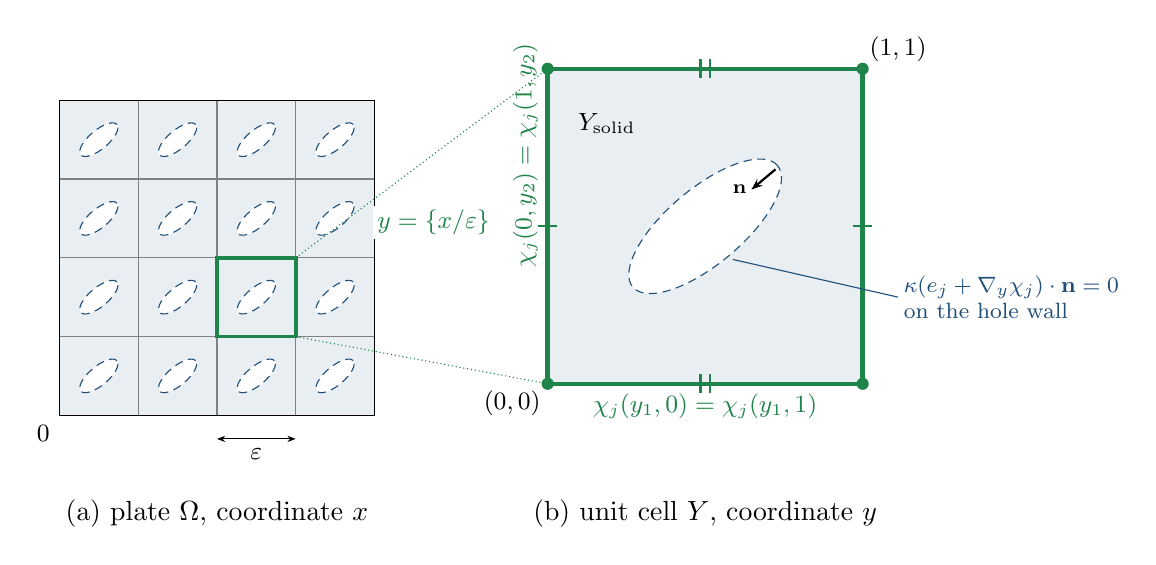
\begin{tikzpicture}[font=\small]
  % ---------------- (a) plate made of cells ----------------
  \begin{scope}
    \fill[solidfill] (0,0) rectangle (4,4);
    \foreach \i in {0,...,3}{\foreach \j in {0,...,3}{\hole{\i+0.5}{\j+0.5}{1}}}
    \draw[gray, thin] (0,0) grid (4,4);
    \draw[per, line width=1.4pt] (2,1) rectangle (3,2);
    \draw (0,0) rectangle (4,4);
    \draw[{Stealth[length=3pt]}-{Stealth[length=3pt]}] (2,-0.3) -- (3,-0.3) node[midway, below] {$\varepsilon$};
    \node[below left] at (0,0) {$0$};
    \node[font=\normalsize] at (2,-1.25) {(a) plate $\Omega$, coordinate $x$};
  \end{scope}
  % zoom lines and change of variable
  \draw[per, thin, densely dotted] (3,2) -- (6.2,4.4);
  \draw[per, thin, densely dotted] (3,1) -- (6.2,0.4);
  \node[per, fill=white, inner sep=1.5pt] at (4.75,2.45) {$y=\{x/\varepsilon\}$};
  % ---------------- (b) unit cell ----------------
  \begin{scope}[xshift=6.2cm, yshift=0.4cm]
    \fill[solidfill] (0,0) rectangle (4,4);
    \hole{2}{2}{4}
    % periodic faces with identification marks
    \draw[per, line width=1.6pt] (0,0) -- (0,4);
    \draw[per, line width=1.6pt] (4,0) -- (4,4);
    \draw[per, line width=1.6pt] (0,0) -- (4,0);
    \draw[per, line width=1.6pt] (0,4) -- (4,4);
    \foreach \x in {0,4}{\draw[per, thick] (\x-0.12,2) -- (\x+0.12,2);}
    \foreach \y in {0,4}{\draw[per, thick] (1.94,\y-0.12) -- (1.94,\y+0.12);
                          \draw[per, thick] (2.06,\y-0.12) -- (2.06,\y+0.12);}
    \foreach \p in {(0,0),(4,0),(0,4),(4,4)}{\fill[per] \p circle (2.2pt);}
    \node[per, rotate=90, above] at (0,2.9) {$\chi_j(0,y_2)=\chi_j(1,y_2)$};
    \node[per, below] at (2,0) {$\chi_j(y_1,0)=\chi_j(y_1,1)$};
    \node[below left=-1pt] at (0,0) {$(0,0)$};
    \node[above right=-1pt] at (4,4) {$(1,1)$};
    \node at (0.75,3.3) {$Y_{\mathrm{solid}}$};
    % insulated hole wall
    \draw[-{Stealth[length=4pt]}, thick] ($(2,2)+(40:{0.3*4})+(-50:0.02)$) ++(220:0.05) -- ++(220:0.4)
       node[left=-2pt, font=\scriptsize] {$\mathbf{n}$};
    \draw[neu, thin] ($(2,2)+(-50:0.55)$) -- (4.45,1.1);
    \node[neu, right, align=left, font=\footnotesize] at (4.4,1.1)
       {$\kappa(e_j+\nabla_y\chi_j)\cdot\mathbf{n}=0$\\on the hole wall};
    \node[font=\normalsize] at (2,-1.65) {(b) unit cell $Y$, coordinate $y$};
  \end{scope}
\end{tikzpicture}
\end{document}
